\documentclass{beamer}

\usetheme{Warsaw}

\usepackage{color}
\usepackage{graphicx}
\usepackage{multirow}
\usepackage[normalem]{ulem}
%\usepackage{soul}
\newcommand{\del}[1]{\sout{#1}}

\def\done{\hfill$\square$}
\def\vgap{\vspace{5mm}}

\newcommand{\red}[1]{\textcolor{red}{#1}}
\def\tabpos{\hspace{4mm} \= \hspace{4mm} \= \hspace{4mm} \= \hspace{4mm} \= \hspace{4mm} \= \hspace{4mm} \= \hspace{4mm} \= \hspace{4mm} \= \hspace{4mm} \kill}

\def\real{\mathbb{R}}

\title{Introduction to Skylines}

\author[]{Yufei Tao \\[2mm]
Department of Computer Science and Technology \\
Chinese University of Hong Kong}

\institute[]
{}

%\date{}

\begin{document}
%-------------------------------------------------------------
    \begin{frame}
        \titlepage
    \end{frame}
%-------------------------------------------------------------
%%-------------------------------------------------------------
%\begin{frame}{Outline}
%    \tableofcontents
%\end{frame}
%%-------------------------------------------------------------
%\section{Problem definitions}
%-------------------------------------------------------------
    \begin{frame}
    \begin{small}
        \begin{definition}[Monotonically increasing function]
            Let $p$ be a $d$-dimensional point in $\real^d$. Let $f: \real^d \rightarrow \real$ a function that calculates a score $f(p)$ for $p$. We say that $f$ is \red{\em monotonically increasing} if the score never decreases when any coordinate of $p$ increases.
        \end{definition}

        For example, $f(x, y) = x + y$ is monotonically increasing but $f(x, y) = x - y$ is not.

        \begin{definition}[Top-1 search]
            Let $P$ be a set of $d$-dimensional points in $\real^d$. Given a monotonically increasing function $f$, a \red{\em top-1 query} finds the point in $P$ that has the smallest score.
        \end{definition}
    \end{small}
    \end{frame}
%-------------------------------------------------------------
%-------------------------------------------------------------
    \begin{frame}{Example}
    \begin{small}
        If $f(x, y) = x + y$, then the top-1 is $p_8$.
        \begin{center}
            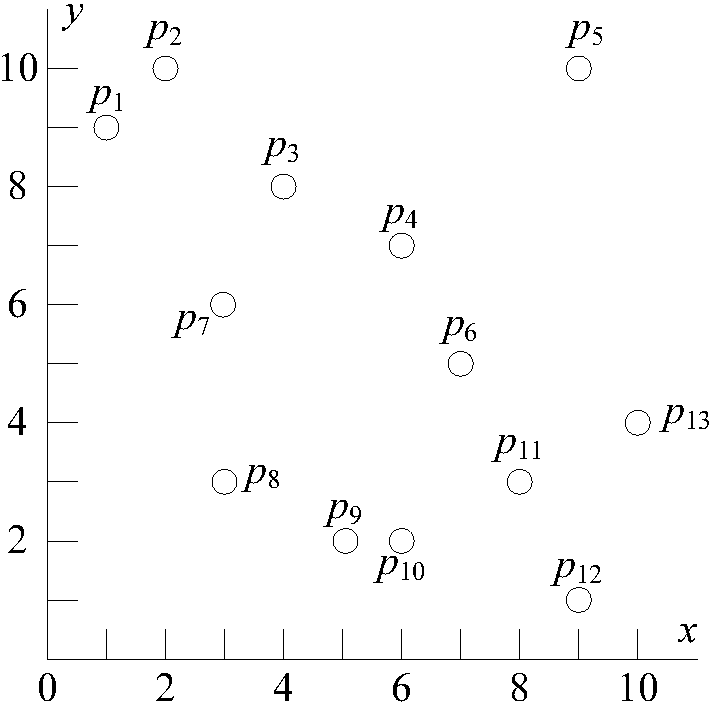
\includegraphics[height=45mm]{./artwork/data.pdf}
        \end{center}
    \end{small}
    \end{frame}
%-------------------------------------------------------------
    \begin{frame}{Applications}
    \begin{small}
		\begin{minipage}{0.48\linewidth}
		    \begin{itemize}
				\item Find the best NBA player according to {\em point} + {\em rebound}.
				\item Find the best hotel according to {\em price} + {\em distance} (say to the town center).
				\item Find the best laptop according to {\em $-$CPU-speed} {\em $-$memory} {\em $-$disk-volume} + {\em price}.
			\end{itemize}
		\end{minipage}
		\begin{minipage}{0.48\linewidth}
        \begin{center}
            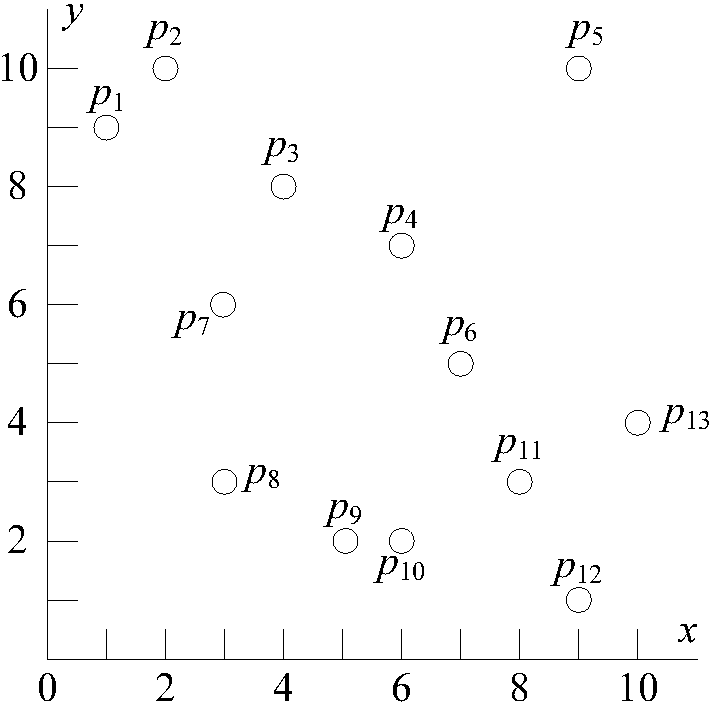
\includegraphics[height=45mm]{./artwork/data.pdf}
        \end{center}
		\end{minipage}
    \end{small}
    \end{frame}
%-------------------------------------------------------------
    \begin{frame}{Drawback of top-1 search}
    \begin{small}
        In general, it is difficult to decide which distance function $f$ should be used. For example, assume that the x-dimension corresponds to the price of a hotel and the y-dimension to its distance to the town center. Why is $f(x, y) = x + y$ a good function to use? Why not $2x + y$, or something more complex like $\sqrt{x} + y^2$?
        \begin{center}
            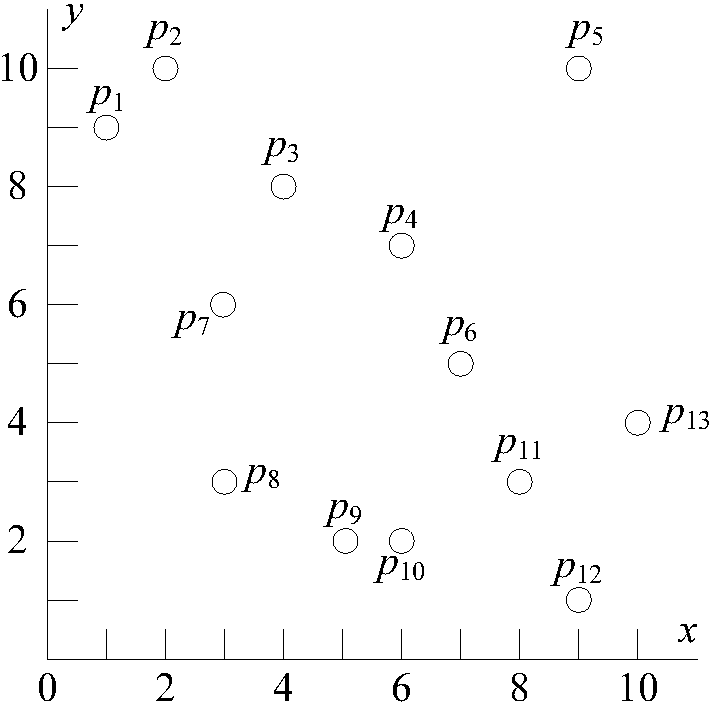
\includegraphics[height=45mm]{./artwork/data.pdf}
        \end{center}
    \end{small}
    \end{frame}
%-------------------------------------------------------------
%-------------------------------------------------------------
    \begin{frame}
    \begin{small}
        The skyline operator remedies the drawback of top-1 search with an interesting idea. Instead of reporting only 1 object, the operator reports a set of objects that are guaranteed to cover the result of \red{any} top-1 query (i.e., \red{regardless of} the query function, as long as it is monotonically increasing!).
    \end{small}
    \end{frame}
%-------------------------------------------------------------
%-------------------------------------------------------------
    \begin{frame}
    \begin{small}
        \begin{definition}[Dominance]
            A point $p_1$ \red{\em dominates} $p_2$ if the coordinate of $p_1$ is smaller than or equal to $p_2$ in all dimensions, and strictly smaller in one dimension.
        \end{definition}

        Note that $p_1$ has a smaller score than $p_2$ with respect to all monotonically increasing function.

        \begin{definition}[Skyline]
            Let $P$ be a set of $d$-dimensional points in $\real^d$ such that no two points coincide with each other. The \red{\em skyline} of $P$ contains all the points that are not dominated by others.
        \end{definition}

        The skyline is also known as {\em pareto set}.
    \end{small}
    \end{frame}
%-------------------------------------------------------------
%-------------------------------------------------------------
    \begin{frame}
    \begin{small}
        The skyline is $\{p_1, p_8, p_9, p_{12}\}$.
        \begin{center}
            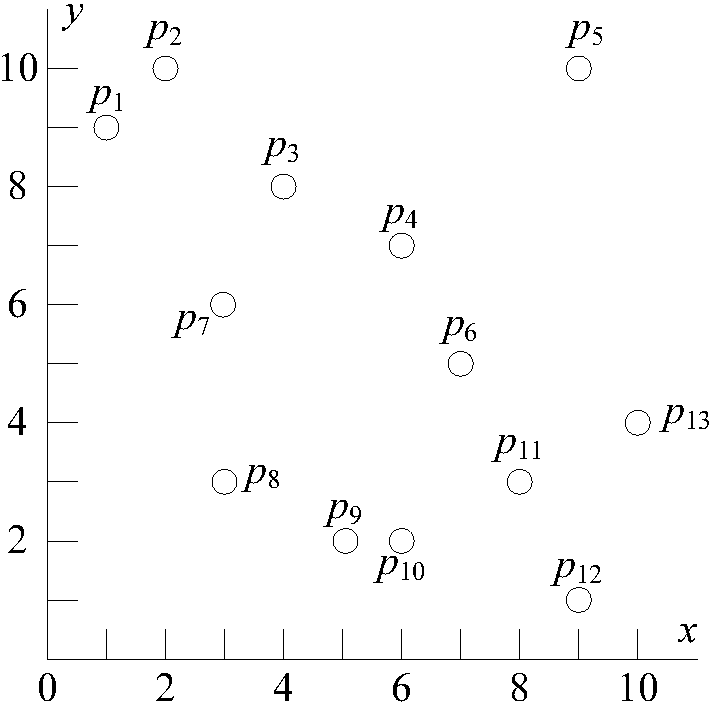
\includegraphics[height=45mm]{./artwork/data.pdf}
        \end{center}
    \end{small}
    \end{frame}
%-------------------------------------------------------------
\begin{frame}{Real example (by courtesy of Donghui Zhang)}
    \begin{small}
		\begin{center}
		\begin{tabular}{c|c|c|c|c}
		    name & point & rebound & assist & steal \\
			\hline
			Tracy McGrady & 2003 & 484 & 448 & 135 \\
			Kobe Bryant & 1819 & 392 & 398 & 86 \\
			Shaquille O'Neal & 1669 & 760 & 200 & 36 \\
			Ming Yao & 1465 & 669 & 61 & 34 \\
			Dwyane Wade & 1854 & 397 & 520 & 121 \\
			Steve Nash & 1165 & 249 & 861 & 74
		\end{tabular}
		\end{center}
    \end{small}
    \end{frame}
%-------------------------------------------------------------
\begin{frame}{Real example}
    \begin{small}
		4D skyline (negate all numbers to be consistent with our earlier definitions):
		\begin{center}
		\begin{tabular}{c|c|c|c|c}
		    name & point & rebound & assist & steal \\
			\hline
			\red{Tracy McGrady} & 2003 & 484 & 448 & 135 \\
			Kobe Bryant & 1819 & 392 & 398 & 86 \\
			\red{Shaquille O'Neal} & 1669 & 760 & 200 & 36 \\
			Ming Yao & 1465 & 669 & 61 & 34 \\
			\red{Dwyane Wade} & 1854 & 397 & 520 & 121 \\
			\red{Steve Nash} & 1165 & 249 & 861 & 74
		\end{tabular}
		\end{center}
    \end{small}
    \end{frame}
%-------------------------------------------------------------
\begin{frame}{Real example}
    \begin{small}
		2D skyline by focusing on the first 2 attributes
		\begin{center}
		\begin{tabular}{c|c|c|c|c}
		    name & point & rebound & \del{assist} & \del{steal} \\
			\hline
			\red{Tracy McGrady} & 2003 & 484 & \del{448} & \del{135} \\
			Kobe Bryant & 1819 & 392 & \del{398} & \del{86} \\
			\red{Shaquille O'Neal} & 1669 & 760 & \del{200} & \del{36} \\
			Ming Yao & 1465 & 669 & \del{61} & \del{34} \\
			\red{Dwyane Wade} & 1854 & 397 & \del{520} & \del{121} \\
			Steve Nash & 1165 & 249 & \del{861} & \del{74}
		\end{tabular}
		\end{center}
    \end{small}
    \end{frame}
%-------------------------------------------------------------
    \begin{frame}
    \begin{small}
        \begin{theorem} \em
            For any monotonically increasing function, the top-1 point is definitely in the skyline. Conversely, every point in the skyline is definitely the top-1 of some monotonically increasing function.
        \end{theorem}

		\begin{center}
            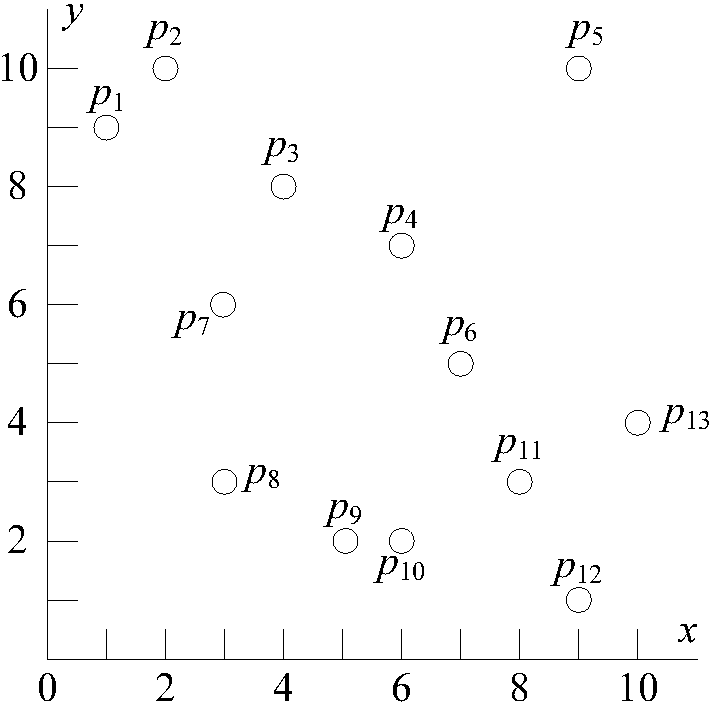
\includegraphics[height=45mm]{./artwork/data.pdf}
        \end{center}
    \end{small}
    \end{frame}
%-------------------------------------------------------------
\begin{frame}
	Next we discuss how to find the skyline of a set $P$ of points efficiently.
\end{frame}
%-------------------------------------------------------------
    \begin{frame}{Naive algorithm}\label{fra:naive}
    \begin{small}
        \begin{tabbing}
            \tabpos

            {\bf algorithm} \texttt{naive} \\
			1.\>	$SKY \leftarrow \emptyset$ \\
            2.\>    {\bf for} each point $p \in P$ \\
            3.\>\>      compare $p$ to all other points in $P$ \\
			4.\>\>		{\bf if} $p$ is not dominated by any other point \\
			5.\>\>\>		add $p$ to the skyline set $SKY$ \\
            6.\>    {\bf return} $SKY$
        \end{tabbing}
    \end{small}
    \end{frame}
%-------------------------------------------------------------
    \begin{frame}
    \begin{small}
        Next, we will describe an algorithm called \red{\em sort first skyline (SFS)} that is fairly efficient on many practical datasets. It works in any dimensionality. The algorithm, however, is heuristic in nature (i.e., it does not have an attractable worst-case performance bound).
    \end{small}
    \end{frame}
%-------------------------------------------------------------
%-------------------------------------------------------------
    \begin{frame}{SFS example}
    \begin{small}
        We will use the following dataset to illustrate the algorithm.
        \begin{center}
            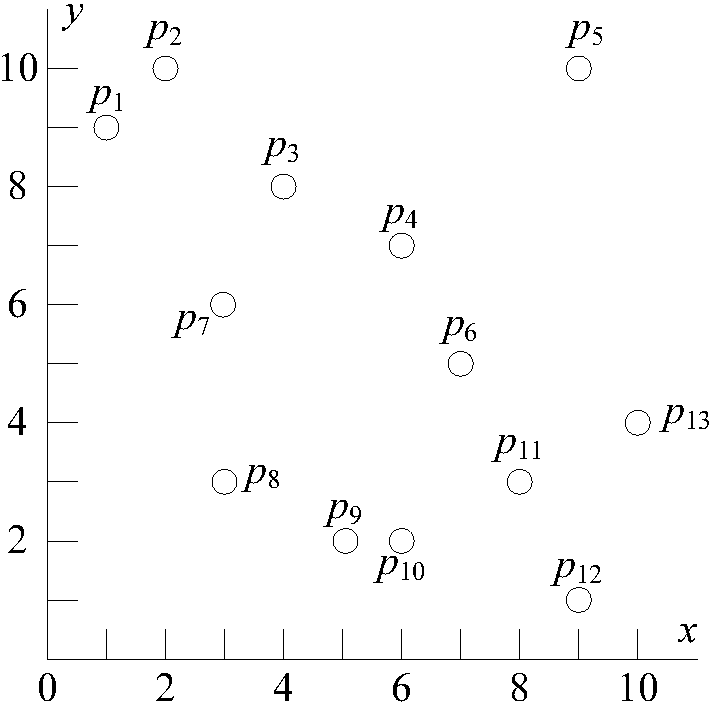
\includegraphics[height=35mm]{./artwork/data.pdf}
        \end{center}
    \end{small}
    \end{frame}
%-------------------------------------------------------------
%-------------------------------------------------------------
    \begin{frame}{SFS example (cont.)}
    \begin{small} \label{fra:sfs-sort}
        First, sort all the points according to an arbitrary monotonically increasing function, e.g., $f(x, y) = x + y$. In case of a tie, the point with a smaller x-coordinate goes first.

		\vgap

		Note that \red{a point can only be dominated by points that rank before it}.

		\vgap

        \begin{minipage}[b]{0.5\linewidth}
            $P = \{(p_8, 6), (p_9, 7), (p_{10}, 8),$ \\
            $(p_1, 9), (p_7, 9), (p_{12}, 10), (p_{11}, 11),$ \\
            $(p_2, 12), (p_3, 12), (p_6, 12), (p_4, 13),$ \\
            $(p_{13}, 14), (p_5, 19)\}$ \vspace{10mm}
        \end{minipage}
        \begin{minipage}[b]{0.45\linewidth}
            \begin{center}
                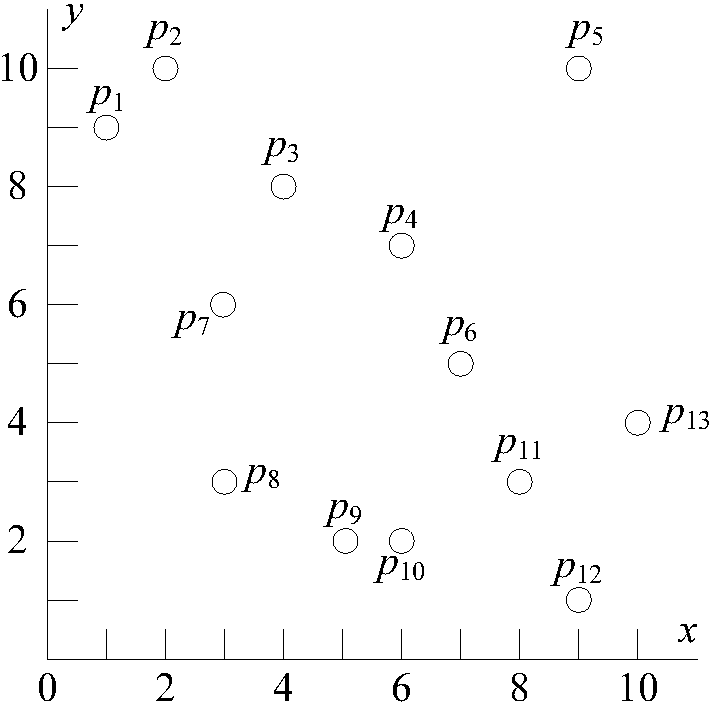
\includegraphics[height=35mm]{./artwork/data.pdf}
            \end{center}
        \end{minipage}
    \end{small}
    \end{frame}
%-------------------------------------------------------------
    \begin{frame}{SFS example (cont.)}
    \begin{small} \label{fra:sfs-sort}
		$p_8$ is definitely in the skyline.

		\vgap

        \begin{minipage}[b]{0.5\linewidth}
            $P = \{\red{(p_8, 6)}, (p_9, 7), (p_{10}, 8),$ \\
            $(p_1, 9), (p_7, 9), (p_{12}, 10), (p_{11}, 11),$ \\
            $(p_2, 12), (p_3, 12), (p_6, 12), (p_4, 13),$ \\
            $(p_{13}, 14), (p_5, 19)\}$ \vspace{10mm}

			$SKY = \{p_8\}$
        \end{minipage}
        \begin{minipage}[b]{0.45\linewidth}
            \begin{center}
                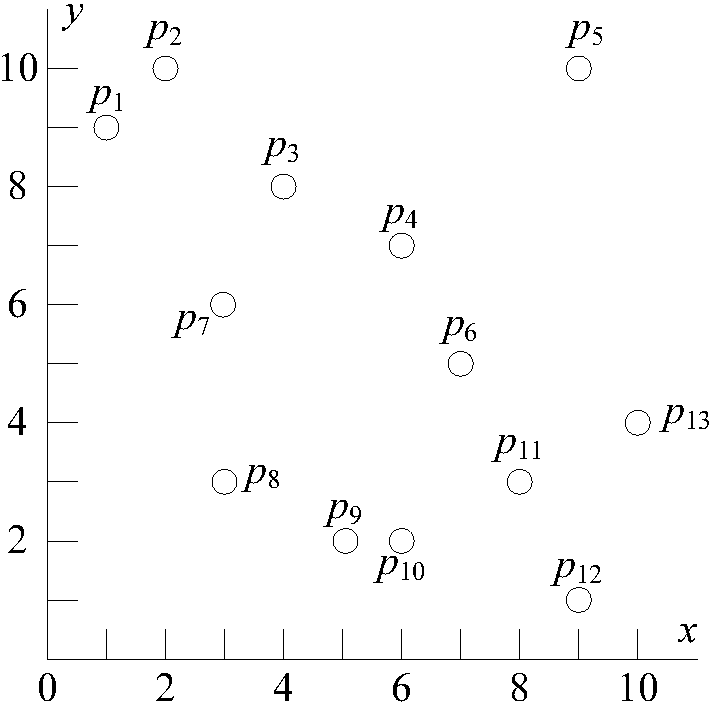
\includegraphics[height=35mm]{./artwork/data.pdf}
            \end{center}
        \end{minipage}
    \end{small}
    \end{frame}
%-------------------------------------------------------------
%-------------------------------------------------------------
    \begin{frame}{SFS example (cont.)}
    \begin{small}
        Next, we scan the rest of the points in the sorted order. For each point $p$:
		\begin{itemize}
		    \item compare it \red{only} to the points in $SKY$;

			\item if it is not dominated by any point in $SKY$, add it to $SKY$.
		\end{itemize}
    \end{small}
    \end{frame}
%-------------------------------------------------------------
    \begin{frame}{SFS example (cont.)}
    \begin{small} \label{fra:sfs-sort}
		$p_9$ is not dominated by $p_8$ (i.e., the only point in $SKY$). Hence, it is added to $SKY$.

		\vgap

        \begin{minipage}[b]{0.5\linewidth}
            $P = \{(p_8, 6), \red{(p_9, 7)}, (p_{10}, 8),$ \\
            $(p_1, 9), (p_7, 9), (p_{12}, 10), (p_{11}, 11),$ \\
            $(p_2, 12), (p_3, 12), (p_6, 12), (p_4, 13),$ \\
            $(p_{13}, 14), (p_5, 19)\}$ \vspace{10mm}

			$SKY = \{p_8, p_9\}$
        \end{minipage}
        \begin{minipage}[b]{0.45\linewidth}
            \begin{center}
                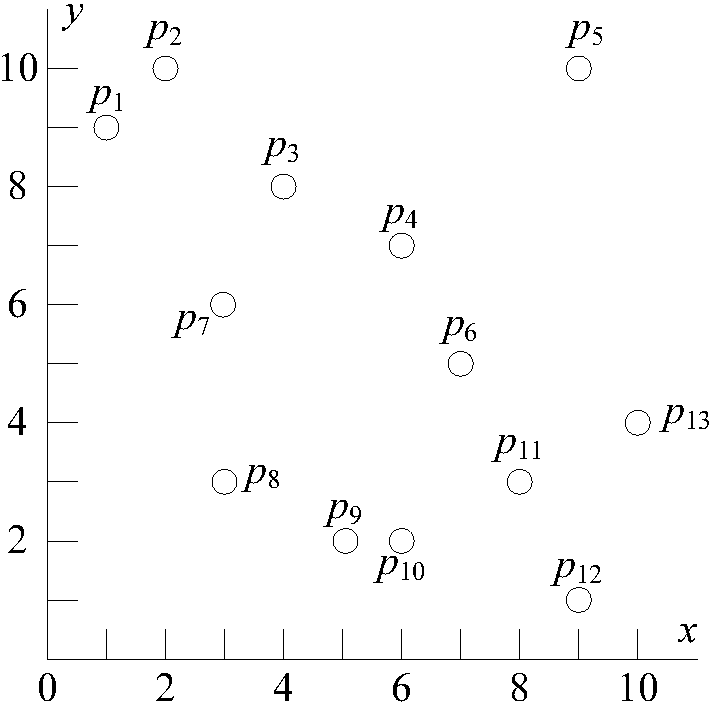
\includegraphics[height=35mm]{./artwork/data.pdf}
            \end{center}
        \end{minipage}
    \end{small}
    \end{frame}
%-------------------------------------------------------------
    \begin{frame}{SFS example (cont.)}
    \begin{small} \label{fra:sfs-sort}
		$p_{10}$ is dominated by $p_9$, and is therefore discarded.

		\vgap

        \begin{minipage}[b]{0.5\linewidth}
            $P = \{(p_8, 6), (p_9, 7), \red{(p_{10}, 8)},$ \\
            $(p_1, 9), (p_7, 9), (p_{12}, 10), (p_{11}, 11),$ \\
            $(p_2, 12), (p_3, 12), (p_6, 12), (p_4, 13),$ \\
            $(p_{13}, 14), (p_5, 19)\}$ \vspace{10mm}

			$SKY = \{p_8, p_9\}$
        \end{minipage}
        \begin{minipage}[b]{0.45\linewidth}
            \begin{center}
                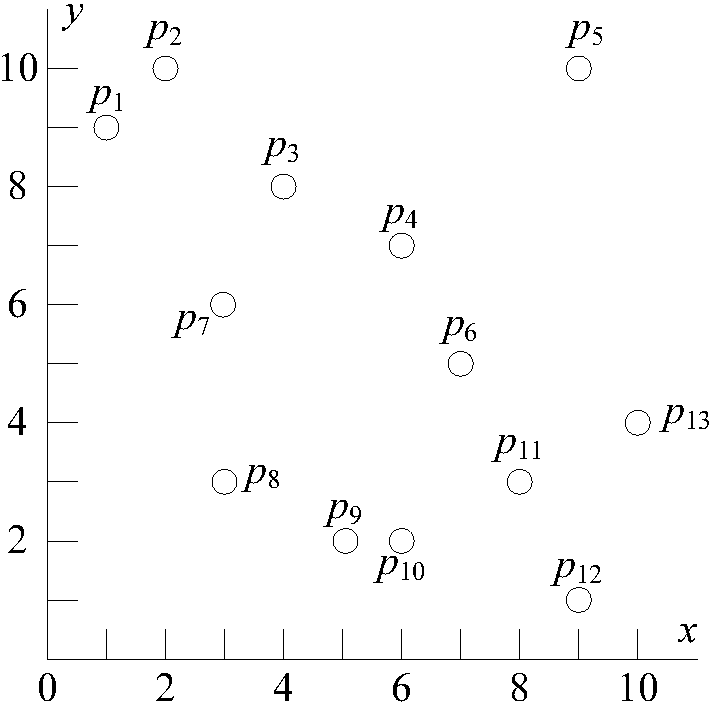
\includegraphics[height=35mm]{./artwork/data.pdf}
            \end{center}
        \end{minipage}
    \end{small}
    \end{frame}
%-------------------------------------------------------------
    \begin{frame}{SFS example (cont.)}
    \begin{small} \label{fra:sfs-sort}
		$p_1$ is added to $SKY$.

		\vgap

        \begin{minipage}[b]{0.5\linewidth}
            $P = \{(p_8, 6), (p_9, 7), (p_{10}, 8),$ \\
            $\red{(p_1, 9)}, (p_7, 9), (p_{12}, 10), (p_{11}, 11),$ \\
            $(p_2, 12), (p_3, 12), (p_6, 12), (p_4, 13),$ \\
            $(p_{13}, 14), (p_5, 19)\}$ \vspace{10mm}

			$SKY = \{p_8, p_9, p_1\}$
        \end{minipage}
        \begin{minipage}[b]{0.45\linewidth}
            \begin{center}
                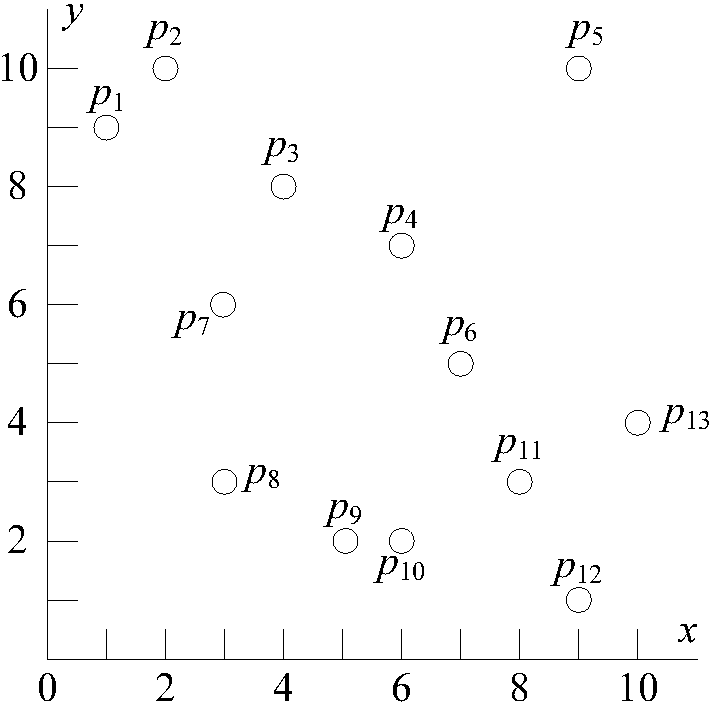
\includegraphics[height=35mm]{./artwork/data.pdf}
            \end{center}
        \end{minipage}
    \end{small}
    \end{frame}
%-------------------------------------------------------------
 \begin{frame}{SFS example (cont.)}
    \begin{small} \label{fra:sfs-sort}
		$p_7$ discarded and $p_{12}$ added to $SKY$.

		\vgap

        \begin{minipage}[b]{0.5\linewidth}
            $P = \{(p_8, 6), (p_9, 7), (p_{10}, 8),$ \\
            $(p_1, 9), \red{(p_7, 9), (p_{12}, 10)}, (p_{11}, 11),$ \\
            $(p_2, 12), (p_3, 12), (p_6, 12), (p_4, 13),$ \\
            $(p_{13}, 14), (p_5, 19)\}$ \vspace{10mm}

			$SKY = \{p_8, p_9, p_1, p_{12}\}$
        \end{minipage}
        \begin{minipage}[b]{0.45\linewidth}
            \begin{center}
                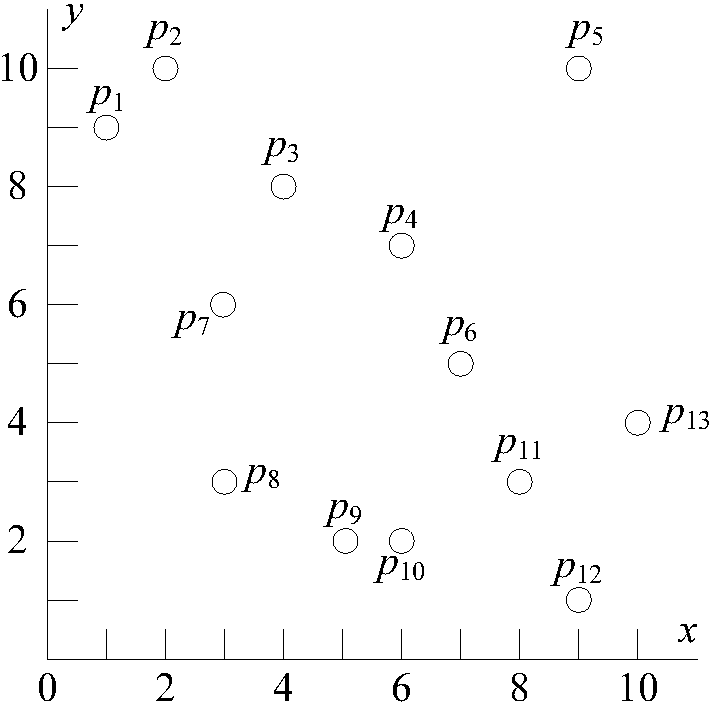
\includegraphics[height=35mm]{./artwork/data.pdf}
            \end{center}
        \end{minipage}
    \end{small}
    \end{frame}
%-------------------------------------------------------------
	\begin{frame}{SFS example (cont.)}
    \begin{small} \label{fra:sfs-sort}
		All other points discarded.

		\vgap

        \begin{minipage}[b]{0.5\linewidth}
            $P = \{(p_8, 6), (p_9, 7), (p_{10}, 8),$ \\
            $(p_1, 9), (p_7, 9), (p_{12}, 10), \red{(p_{11}, 11)},$ \\
            $\red{(p_2, 12), (p_3, 12), (p_6, 12), (p_4, 13),}$ \\
            $\red{(p_{13}, 14), (p_5, 19)}\}$ \vspace{10mm}

			$SKY = \{p_8, p_9, p_1, p_{12}\}$
        \end{minipage}
        \begin{minipage}[b]{0.45\linewidth}
            \begin{center}
                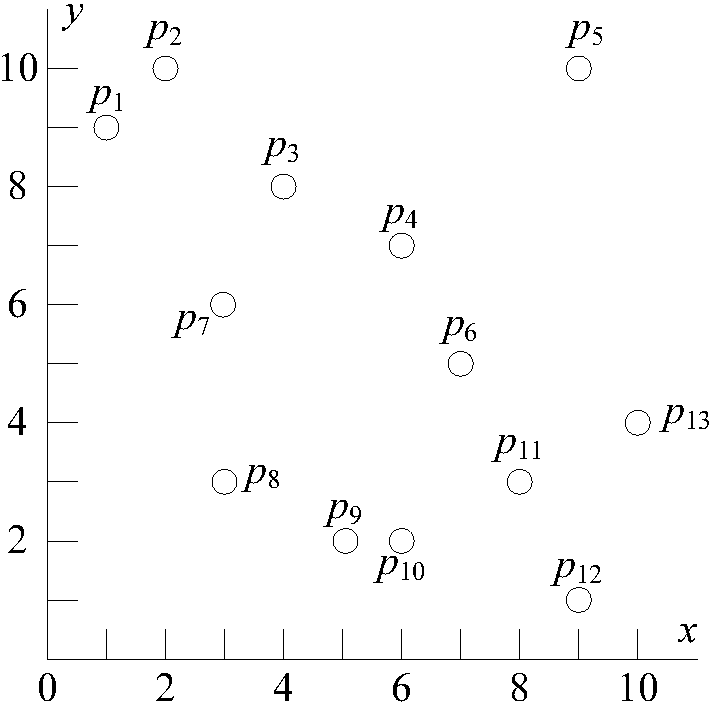
\includegraphics[height=35mm]{./artwork/data.pdf}
            \end{center}
        \end{minipage}
    \end{small}
    \end{frame}
%-------------------------------------------------------------
\begin{frame}{SFS running time}
    \begin{small} \label{fra:sfs-sort}
		\begin{itemize}
		    \item Let $k$ be the number of points in the skyline.
			\item Each point is compared to at most $k$ points.
			\item There are $n$ points in total.
			\item Hence the total time is $O(nk)$.
			\item The initial sorting takes $O(n \lg n)$ time.
		\end{itemize}
		Total: $O(n \lg n + nk)$.
    \end{small}
    \end{frame}
%-------------------------------------------------------------
\begin{frame}{SFS running time}
    \begin{small} \label{fra:sfs-sort}
		\begin{itemize}
		    \item From the previous slide: $O(n \lg n + nk)$.
			\item Efficient if $k$ is small (true in practice when the dimensionality is low).
			\item How about the worst case?
		\end{itemize}
    \end{small}
    \end{frame}
%-------------------------------------------------------------
\begin{frame}{SFS worst case}
    \begin{small} \label{fra:sfs-sort}
		$k = n$
		\begin{center}
            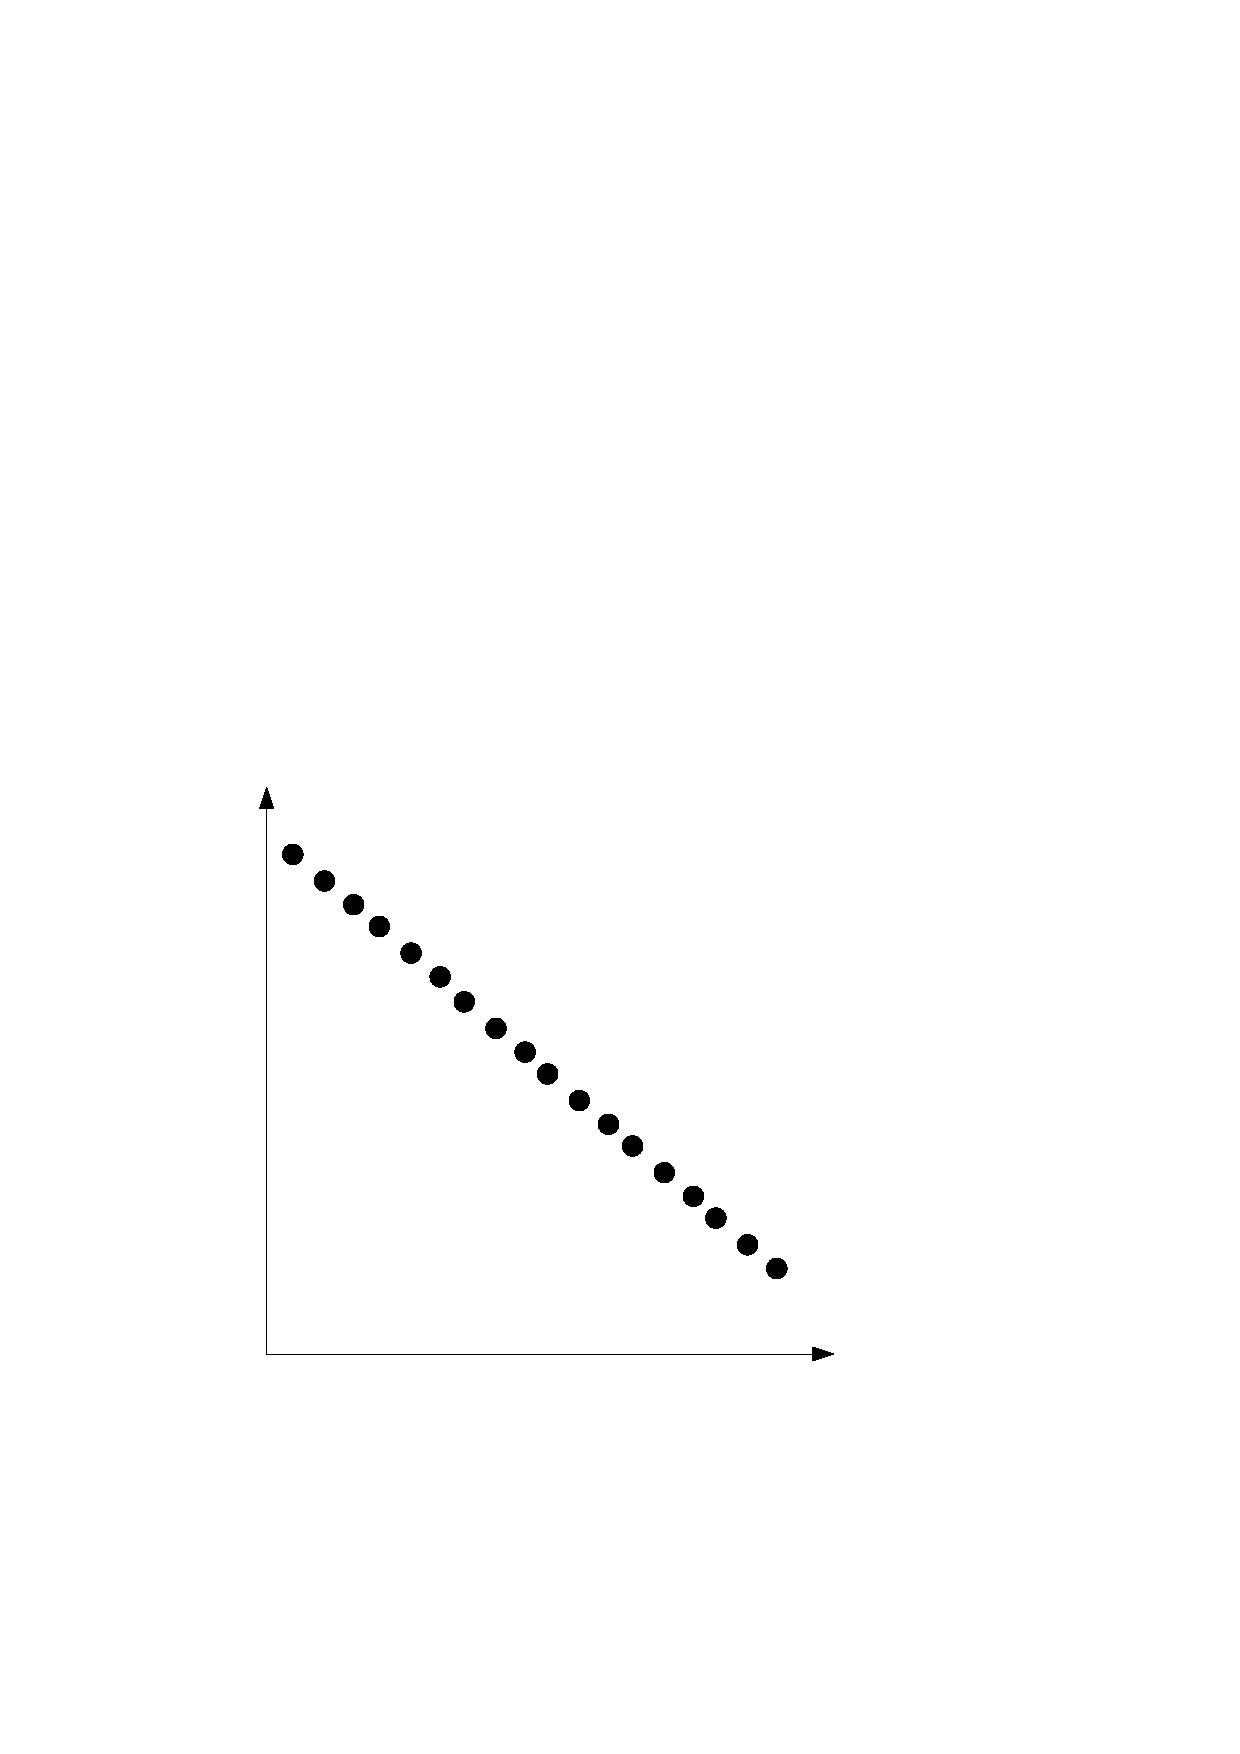
\includegraphics[height=35mm]{./artwork/worst.pdf}
        \end{center}

		Running time = $O(n \lg n + n^2) = O(n^2)$.
    \end{small}
    \end{frame}
%-------------------------------------------------------------
\begin{frame}{}
    \begin{small} \label{fra:sfs-sort}
		Next, we will present two faster algorithms for solving the skyline problem in 2d and 3d, respectively. Both algorithm terminate in $O(n \log n)$ time.
    \end{small}
    \end{frame}
%-------------------------------------------------------------
\begin{frame}{2-d} \label{fra:2d-sort}
\begin{small}
    Assume that $P$ has been sorted in ascending order of their x-coordinates (which can be done in $O(n \log n)$ time). If two points have the same x-coordinate, rank the one with a smaller y-coordinate first. Consider any point $p \in P$. Let $S$ be the set of points that rank before $P$. Observe:
    \begin{itemize}
        \item No point that ranks \red{after} $p$ can possibly dominate $p$.

        \item Some point in $S$ dominates $p$, if and only if the smallest y-coordinate of the points in $S$ is \red{no greater than} the y-coordinate of $p$.
    \end{itemize}
\end{small}
\end{frame}
%-------------------------------------------------------------
\begin{frame}{2-d (cont.)}
\begin{small}
    \begin{center}
        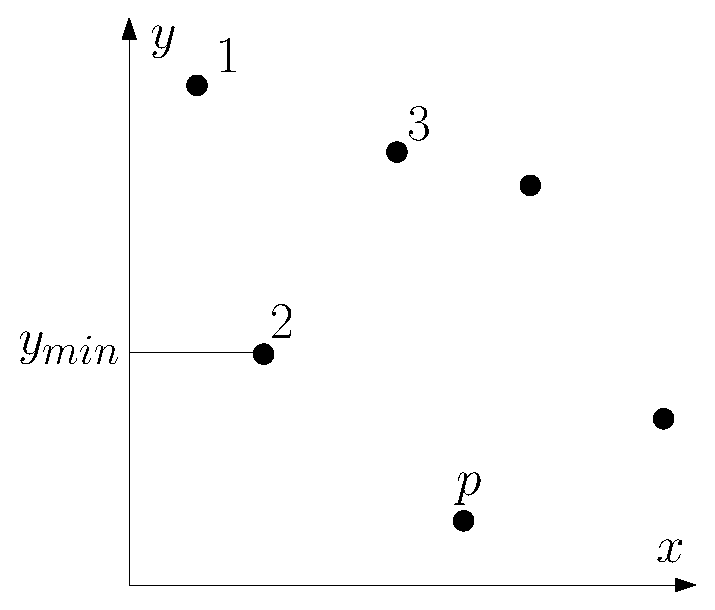
\includegraphics[height=30mm]{./artwork/2d.eps}
    \end{center}
\end{small}
\end{frame}
%-------------------------------------------------------------
\begin{frame}{Pseudocode of the 2-d algorithm}
\begin{small}
    \begin{tabbing}
        \tabpos

        {\bf algorithm} \texttt{2d-skyline} \\
        1.\>    sort the dataset $P$ as described in Slide~\ref{fra:2d-sort} \\
        2.\>    $SKY = \emptyset, y_{min} = \infty$ \\
        2.\>    {\bf for} each point $p \in P$ in the sorted order \\
        3.\>\>      {\bf if} the y-coordinate $p[y]$ of $p$ is smaller than $y_{min}$ \\
        4.\>\>\>        add $p$ to $SKY$, and $y_{min} = p[y]$ \\
        5.\>    {\bf return} $SKY$
    \end{tabbing}

    Line 1 takes $O(n\log n)$ time, whereas Lines 2-4 essentially scan the entire $P$ only once in $O(n)$ time. Hence, the overall cost is $O(n\log n)$.
\end{small}
\end{frame}
%-------------------------------------------------------------
\begin{frame}{3-d}\label{fra:3d-sort}
\begin{small}
    Again, sort $P$ in ascending order of their x-coordinates. Break ties by putting the point with a smaller y-coordinate first, and if there is still a tie, the point with a smaller z-coordinate ranks first.

    \vgap

    Consider any point $p \in P$. Let $S$ be the set of points that rank before $P$. Observe:
    \begin{itemize}
        \item (Same as 2-d) no point that ranks {\em after} $p$ can possibly dominate $p$.

        \item Let $SKY_{yz}(S)$ be the skyline of the \red{projections} of (the points of) $S$ in the y-z plane. Some point in $P$ dominates $p$ in the x-y-z space, if and only if a point of $SKY_{yz}(S)$ dominates $p$ in the y-z plane.
    \end{itemize}
\end{small}
\end{frame}
%-------------------------------------------------------------
\begin{frame}{3-d (cont.)}
\begin{small}
    \begin{example}
        Assume $SKY_{yz}(S)$ includes points 1, 2, 3, 4, 5. As no point of $SKY_{yz}(S)$ dominates $p$ in the y-z plane, we can assert that $p$ is definitely in the skyline (of the original space).
    \begin{center}
        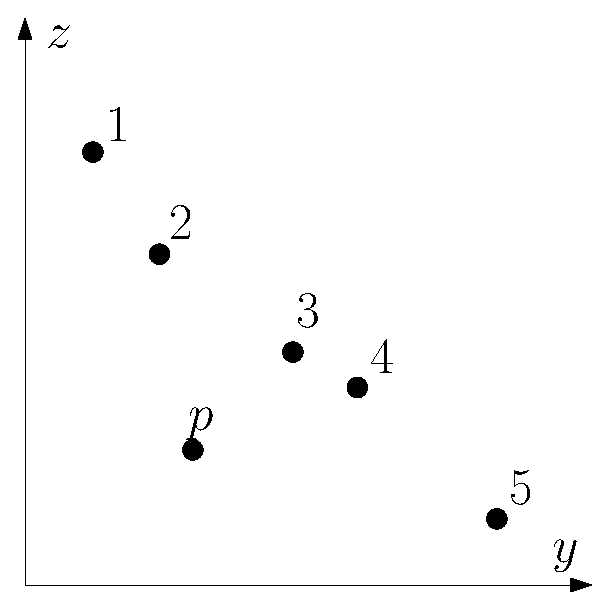
\includegraphics[height=30mm]{./artwork/3d.eps}
    \end{center}
    \end{example}
\end{small}
\end{frame}
%-------------------------------------------------------------
\begin{frame}{3-d (cont.)}
\begin{small}
    $SKY_{yz}(S)$ is a 2-d skyline. In general, a 2-d skyline is a \red{staircase}. Namely, if we walk along the skyline towards the direction of ascending x-coordinates, the y-coordinates of the points keep decreasing.
    \begin{center}
        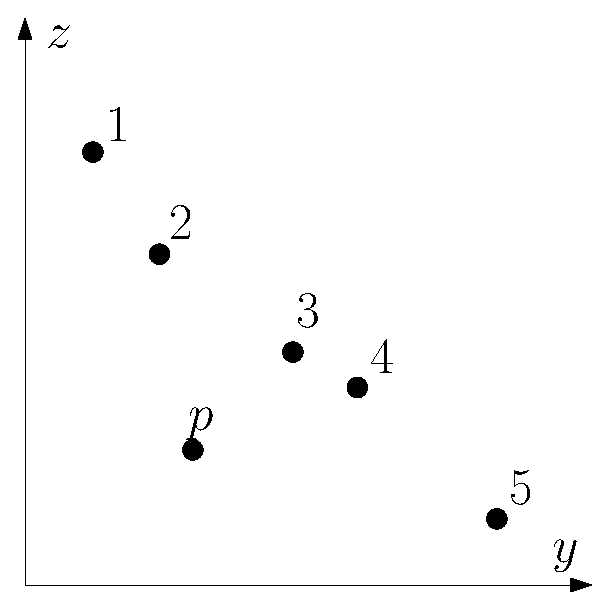
\includegraphics[height=30mm]{./artwork/3d.eps}
    \end{center}
\end{small}
\end{frame}
%-------------------------------------------------------------
\begin{frame}{3-d (cont.)}\label{fra:3d-tree}
\begin{small}
    Let us index the points of $SKY_{yz}(S)$ by their y-coordinates using a binary tree (or a B-tree with a constant $B \ge 4$). Two operations can be done efficiently:
    \begin{itemize}
        \item \red{Detect} if a point $p$ is dominated by any point in $SKY_{yz}(S)$ (in the y-z plane).

        \item \red{Remove} all points of $SKY_{yz}(S)$ dominated by $p$ (in the y-z plane).
    \end{itemize}

    We will show that each detection can be done in $O(\log n)$ time, while removal in $O(k \log n)$ time, where $k$ is the number of points removed.
\end{small}
\end{frame}
%-------------------------------------------------------------
\begin{frame}{3-d (cont.)}
\begin{small}
    Detection is based on the observation that $p$ is dominated by some point in $SKY_{yz}(S)$ if and only if $p$ is dominated by the predecessor of $p$ in $SKY_{yz}(S)$ on the y-dimension. For example, the predecessor is point 2 in the figure below.
    \begin{center}
        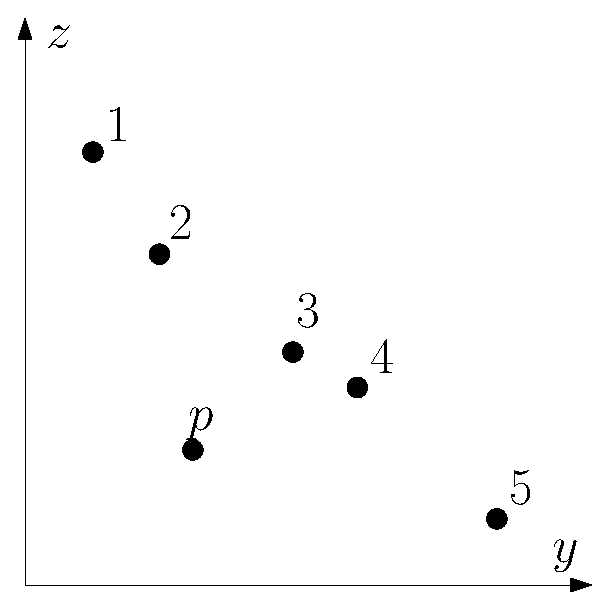
\includegraphics[height=30mm]{./artwork/3d.eps}
    \end{center}
    Finding the predecessor takes $O(\log n)$ time using the binary tree.
\end{small}
\end{frame}
%-------------------------------------------------------------
\begin{frame}{3-d (cont.)}
\begin{small}
    To remove the points of $SKY_{yz}(S)$ dominated by $p$ (in the y-z plane), we first find the successor, say $p'$, of $p$ in $SKY_{yz}(S)$ on the y-dimension. If $p$ dominates $p'$, remove $p'$ and set $p'$ to its own successor. Repeat this until $p$ no longer dominates $p'$. In the figure below, $p'$ iterates through points 3 and 4.
    \begin{center}
        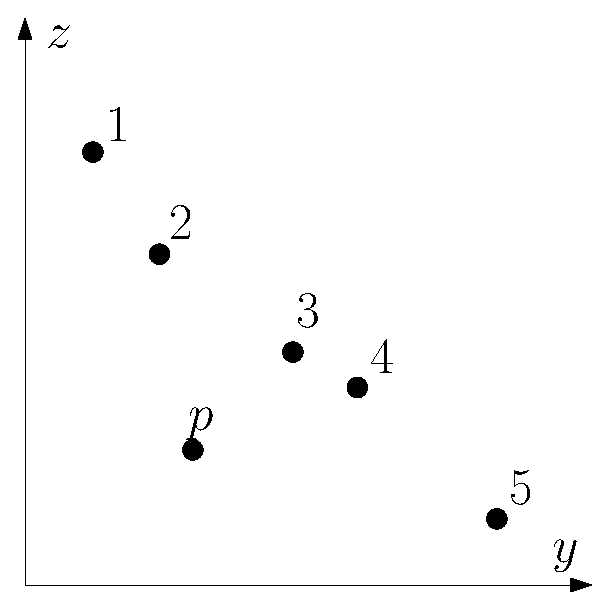
\includegraphics[height=30mm]{./artwork/3d.eps}
    \end{center}
    Finding a successor and removing a point take $O(\log n)$ time.
\end{small}
\end{frame}
%-------------------------------------------------------------
\begin{frame}{Pseudocode of the 3-d algorithm}
\begin{small}
    \begin{tabbing}
        \tabpos

        {\bf algorithm} \texttt{3d-skyline} \\
        1.\>    sort the dataset $P$ as described in Slide \ref{fra:3d-sort} \\
        2.\>    $SKY = \emptyset$ \\
        3.\>    let $T$ be the binary tree as mentioned in Slide~\ref{fra:3d-tree} \\
        4.\>    {\bf for} each point $p \in P$ in the sorted order \\
        5.\>\>      {\bf if} $p$ is not dominated by any point of $T$ in the y-z plane {\bf then} \\
        6.\>\>\>        add $p$ to $SKY$ \\
        7.\>\>\>        remove from $T$ all points dominated by $p$ in the y-z plane \\
        8.\>    {\bf return} $SKY$
    \end{tabbing}

    The detection at Line 5 is performed $n$ times, and thus, requires $O(n \log n)$ time in total. On the other hand, each point is inserted and removed in $T$ at most once. Hence, all the insertions and deletions entail $O(n \log n)$ time.
\end{small}
\end{frame}
%-------------------------------------------------------------
\begin{frame}{Remark}
\begin{small}
    In general, the skyline problem can be settled in $O(n \log^{d-2} n)$ when the dimensionality $d$ is at least 3. The algorithm for $d \ge 4$, however, is quite theoretical, and may not be as efficient as the heuristic algorithm SFS in practice.
\end{small}
\end{frame}
%-------------------------------------------------------------
\end{document}